\begin{figure*}[!ht]
    \centering
    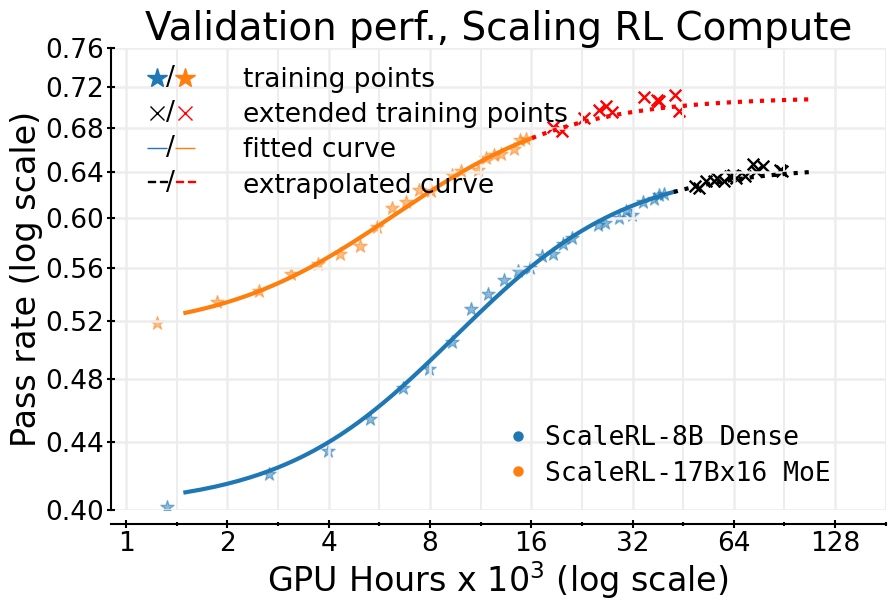
\includegraphics[width=0.54\textwidth]{paper_figs/100k.png}
    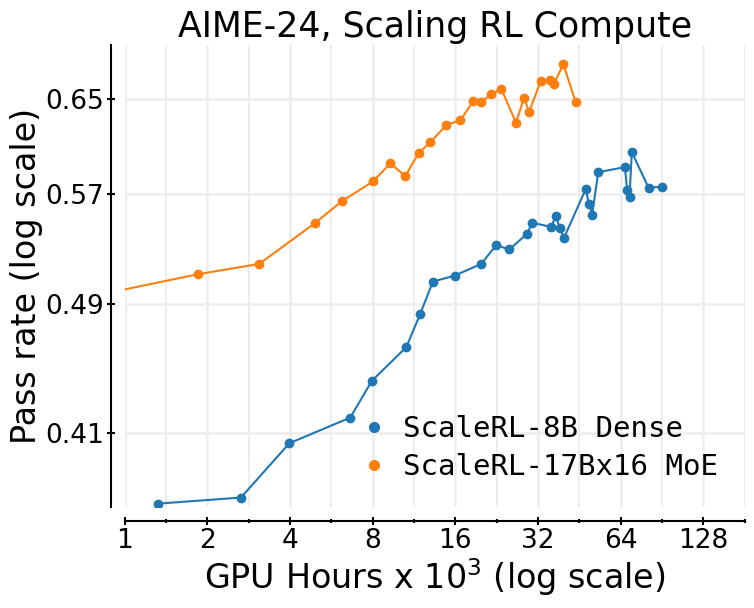
\includegraphics[width=0.45\textwidth]{paper_figs/100k_aime24.png} 
    \caption{ \textbf{Predicatably Scaling RL compute to 100,000 GPU Hours}
    \small{(a) 
    We run \scalerl\ for $100\text{k}$ GPU hours on an 8B dense model, and $50\text{k}$ GPU hours on a 17Bx16 MoE (Scout).
    We fit a sigmoid curve~(\Cref{eq:sigmoid_law}) on pass rate ($\text{mean}@16$) on \emph{iid} validation dataset up to $50\text{k}$ (and $16\text{k})$ GPU hours and extrapolate to $100\text{k}$ (and $45\text{k})$ on the 8B (Scout MoE) models respectively. We trained for $7400$ steps for 8B and $7100$ steps for Scout, which is $3.5\times$ larger than ProRL~\citep{prorl}. The extrapolated curve ($\times$ markers) closely follows extended training, demonstrating both stability at large compute and predictive fits--establishing \scalerl\ as a reliable candidate for RL scaling.
    (b) \textbf{Downstream evaluation on AIME-24} shows a consistent scaling trend for \scalerl, thus generalizing beyond the training data distribution. Moreover, scaling model size substantially improves the downstream and asymptotic RL performance.}
    }
    \label{fig_100k_main}
\end{figure*}

\section{Introduction}
\label{sec:intro}



Scaling reinforcement learning (RL) compute is emerging as a critical paradigm for advancing large language models (LLMs). While pre-training establishes the foundations of a model; the subsequent phase of RL training unlocks many of today’s most important LLM capabilities, from test-time thinking~\citep{openai-o1, guo2025deepseek} to agentic capabilities~\citep{team2025kimi2}. For instance, Deepseek-R1-Zero used 100,000 H800 GPU hours for RL training -- 3.75\% of its pre-training compute~\citep{guo2025deepseek}. This dramatic increase in RL compute is amplified across frontier LLM generations, with more than 10$\times$ increase from o1 to o3~\citep{OpenAI.o3.2025} and a similar leap from Grok-3 to Grok-4~\citep{grok4}.


While RL compute for LLMs has scaled massively, our understanding of \emph{how} to scale RL has not kept pace; the methodology remains more \emph{art} than science. Recent breakthroughs in RL are largely driven by isolated studies on novel algorithms (e.g., \citet[DAPO,][]{yu2025dapo}) and model-specific training reports, such as, \citet{minimax_m1} and Magistral~\citep{rastogi2025magistral}. Critically, these studies provide \emph{ad-hoc} solutions tailored to specific contexts, but not \emph{how} to develop RL methods that scale with compute. This lack of scaling methodology stifles research progress: with no reliable way to identify promising RL candidates \emph{a priori}, progress is tied to large-scale experimentation that sidelines most of the academic community. 


This work lays the groundwork for science of RL scaling by borrowing from the well-established concept of \emph{scaling laws} from pre-training. While pre-training has converged to algorithmic recipes that scale \emph{predictably} with compute~\citep{kaplan2020scaling, hoffmann2022training, owen2024predictable}, the RL landscape lacks a clear standard.
As a result, RL practitioners face an overwhelming array of design choices, leaving the fundamental questions of \emph{how} to scale and \emph{what} to scale unanswered.
To address these questions, we establish a predictive framework for RL performance using a sigmoid-like saturating curve between the expected reward ($R_C$) on an \emph{iid} validation set and training compute ($C$):
\begin{align}
\boxed{\overbrace{R_C - R_0}^{\text{Reward Gain}} = \overbrace{(A - R_0)}^{\text{Asymptotic Reward Gain}}\times \frac{1}{\underbrace{1 + (C_\text{mid}/C)^{B}}_{\text{Compute Efficiency}}}} && \text{\emph{(fixed model and training data)}}
\label{eq:sigmoid_law}
\end{align}

\begin{figure*}[t]
    \centering
    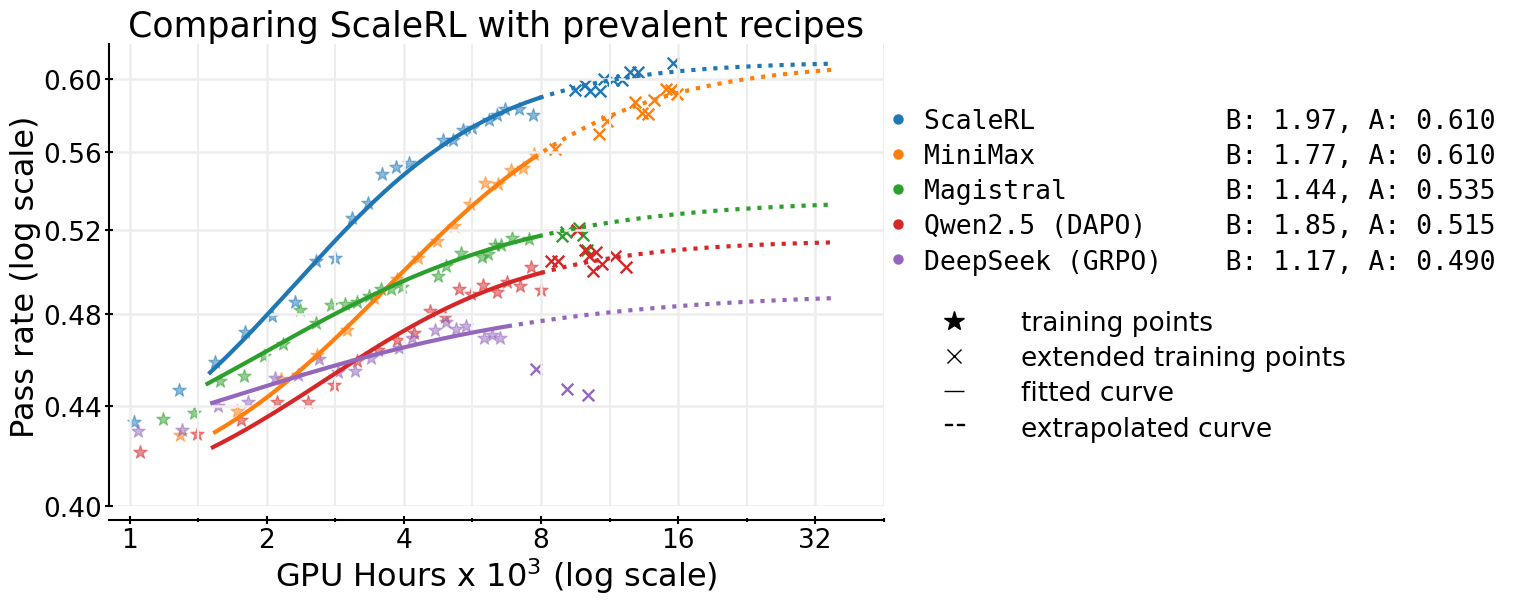
\includegraphics[width=1\textwidth]{paper_figs/prevalent_methods.png} \caption{\small{\textbf{\scalerl\ is more scalable than prevalent RL methods}.  We fit sigmoid curves (Equation~\ref{eq:sigmoid_law}) on \emph{iid} validation dataset to commonly-used training recipes like DeepSeek (GRPO)~\citep{guo2025deepseek}, Qwen-2.5 (DAPO)~\citep{yu2025dapo}, Magistral~\citep{rastogi2025magistral}, and Minimax-M1~\citep{minimax_m1}, and compare them with \scalerl. \scalerl\ surpasses all other methods, achieving an asymptotic reward of $A=0.61$. Stars denote evaluation points; solid curves show the fitted curve over the range used for fitting; dashed curves extrapolate beyond it. We validate the predictability by running each method for longer (``$\times$'' markers), which align closely with the extrapolated curves for stable recipes like \scalerl\ and MiniMax. Further description of the individual recipes compared are given in Appendix~\ref{appendix:prevelant_methods}.}}
    \label{fig:prevelant_methods}
\end{figure*}

where $0 \le A \le 1$ represents the asymptotic pass rate, $B > 0$ is a scaling exponent that determines the compute efficiency, and $C_\text{mid}$ sets the midpoint of the RL performance curve. A schematic interpretation of these parameters is provided in \Cref{fig:interpreting_fit}.

This framework in \Cref{eq:sigmoid_law} allows researchers to extrapolate performance from lower-compute runs to higher compute budgets, enabling them to evaluate scalability of RL methods without incurring the compute cost of running every experiment to its computational limit.




Guided by this framework, we develop \scalerl, an RL recipe that scales \emph{predictably} with compute.
In a massive \textbf{100,000 GPU-hours training run},  we show that \scalerl's performance closely matches the scaling curve predicted by our framework~(Figure~\ref{fig_100k_main}). Critically, scaling curves extrapolated from only the initial stages of training closely match the final observed performance, confirming the predictive ability of our framework to extreme compute scales.


The design of \scalerl\ is grounded in a comprehensive empirical study of RL scaling that spanned over \textbf{400,000 GPU-hours} (on Nvidia GB200 GPUs). This study explored numerous design choices at an 8B model parameters scale, where individual runs use up to 16,000 GPU-hours, making them \textbf{6$\times$ cheaper} than experimenting at our largest training run scale. This investigation yielded three key principles:
\begin{itemize}[leftmargin=2em]
    \item \textbf{RL Performance Ceilings are Not Universal}: As we scale training compute for different methods, they encounter different ceilings on their achievable performance ($A$). This limit can be shifted by choices such as the loss type and batch size.
    \item \textbf{Embracing the Bitter Lesson}: Methods that appear superior at small compute budgets can be worse when extrapolated to large-compute regimes~(\Cref{fig:prevelant_methods}). We can still identify scalable methods by estimating the scaling parameters ($A$, $B$) from the early training dynamics using our framework~(\Cref{eq:sigmoid_law}).
    \item \textbf{Re-evaluating Common Wisdom}: Common interventions thought to improve peak performance~(e.g., loss aggregation, data curriculum, length penalty, advantage normalization) mainly adjust compute efficiency~($B$), while not changing the performance ceiling considerably. 
\end{itemize}

Based on these insights, \scalerl\ achieves \emph{predictable} scaling by integrating existing methods, rather than inventing novel methods. Specifically, \scalerl\ combines asynchronous Pipeline-RL setup~(\S\ref{sec:infra}), forced length interruptions, truncated importance sampling RL loss (CISPO), prompt-level loss averaging, batch-level advantage normalization, FP32 precision at logits, zero-variance filtering, and No-Positive-Resampling -- with each component's contribution validated in a leave-one-out ablation, consuming 16,000 GPU-hours per run.


\scalerl\ not only scales \emph{predictably} but also establishes a new \textbf{state-of-the-art}~(\Cref{fig:prevelant_methods}) -- it achieves higher asymptotic performance and compute efficiency compared to established RL recipes.  Moreover, \scalerl\ maintains predictable scaling when increasing compute across multiple training axes (\S~\ref{sec:diff_axes}) -- including 2.5$\times$ larger batch sizes, longer generation lengths up to 32,768 tokens, multi-task RL using math and code, and larger MoE (Llama-4 17B$\times16$); with benefits that consistently transfer to downstream tasks. Overall, this work establishes a rigorous methodology for cost-effectively predicting the scalability of new RL algorithms. 